\documentclass[utf8]{beamer}
\mode<presentation>
\usepackage[spanish]{babel}
\usepackage{multicol}
\useoutertheme{infolines} 
\usepackage{graphicx}
\usetheme{boxes}

\definecolor{lightblue}{rgb}{0,.5,1}
%\beamertemplateshadingbackground{lightblue!50}{lightblue!50}
%\setbeamercovered{transparent}

\usebackgroundtemplate{
\includegraphics[width= \paperwidth, height=\paperheight]{fondo.jpg}}

\begin{document}
	\begin{frame}
		\color{red}\textbf{\begin{center}{\Huge{¡Entregando Tareas!}}\end{center}}			
		\pause
		\begin{center} 
				 
\includegraphics[width=0.5\textwidth]{document01.png} %Midifico el width para cambiar el tamaño%
		\end{center}
	\end{frame}
\usebackgroundtemplate{
\includegraphics[width= \paperwidth, height=\paperheight]{fondo.jpg}}
	\begin{frame}	 	
		\color{red}\textbf{\begin{center}{\Huge{Desarrolladores}}\end{center}}
		\color{black}
		\begin{center}\huge{ 
			\pause
			- Ana Arias\\
			\pause
 			- César San Lucas
			\pause
		}
			\normalsize
			\vspace{9mm}
			\\Lenguajes de Programación
			\\2012 - II Término			
		\end{center}				
	\end{frame}
	\begin{frame}
		\begin{center} 
			 
\includegraphics[width=0.8\textwidth]{funcionalidades.jpg}
		\end{center}
	\end{frame}
	\begin{frame}
		\frametitle{
	 		\begingroup
				\begin{center}
					\normalsize
					\color{blue}El aprender resolviendo tu tarea...
					\pause
					\newline
					 Nunca había sido tan divertido
					\pause
				\end{center}
			\endgroup
		}
		\begin{center}
			\begin{itemize}
				\vspace{-1cm}
				\item\textbf{PONDRÁS A PRUEBA QUE TAN BUENA MEMORIA TIENES}
				\newline
				Escucharás  una secuencia de números y letras, tendrás que memorizarlos e ingresarlos digitando dicha secuencia corectamente.
			\end{itemize}
		\end{center}
		\begin{center} 
			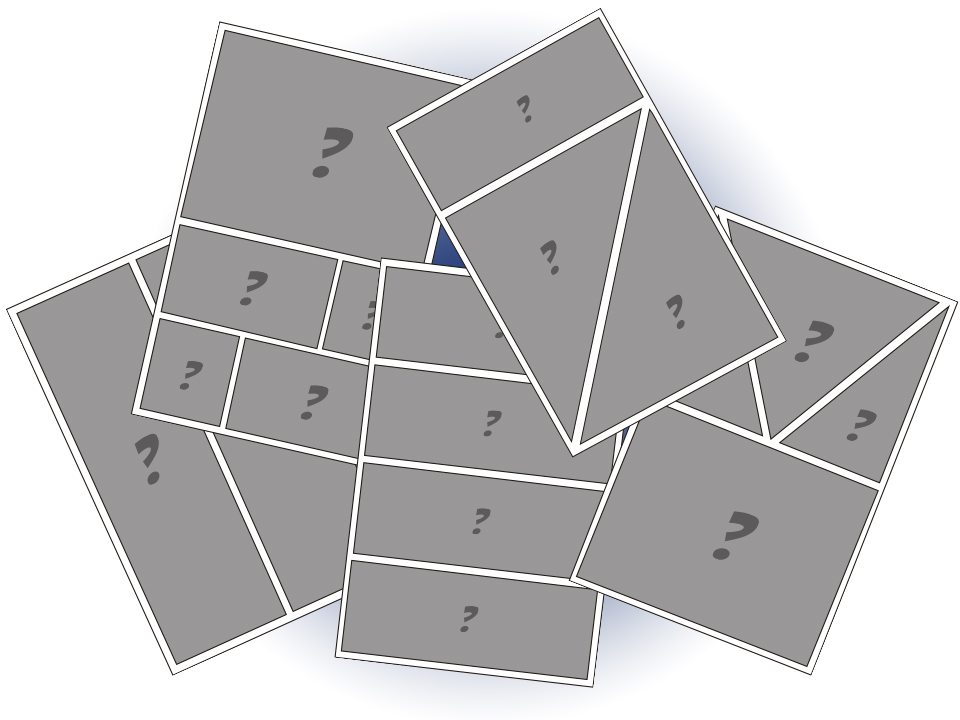
\includegraphics[width=0.4\textwidth]{plantillas.jpg}
		\end{center}
	\end{frame}
	\begin{frame}
		\frametitle{
	 		\begingroup
				\begin{center}
				\color{blue}El aprender resolviendo tu tarea...
					\pause
					\newline
					 Nunca había sido tan divertido
					\pause
				\end{center}
			\endgroup
		}
		\begin{center}
			\vspace{-1cm}
			\begin{itemize}
				\item\textbf{LISTA DE TAREAS PERSONALIZADAS}
				\newline
				Proporcionamos una lista con varios ejercicios dependiendo de tu edad y nivel de educación
 				en el que te encuentras, la idea es que luego de completar tu tarea la entregues para lo cual 
				tendrás que completar un divertido juego con diversos obstáculos y un objetivo que cumplir con lo
 				que también pondrás a prueba tus habilidades motrices.	
			\end{itemize}
		\end{center}
		\begin{center}
			\begingroup
				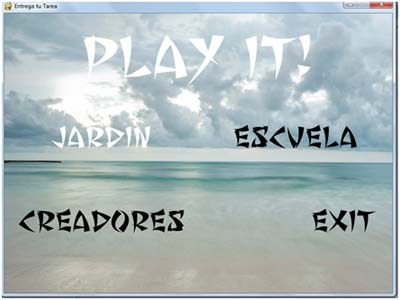
\includegraphics[width=0.3\textwidth]{principal.jpg}
			\endgroup
		\end{center}
	\end{frame}	
	\begin{frame}
		\begin{center} 
			 
\includegraphics[width=0.9\textwidth]{demo.jpg}
		\end{center}
	\end{frame}
	\begin{frame}
		\begin{center} 
			 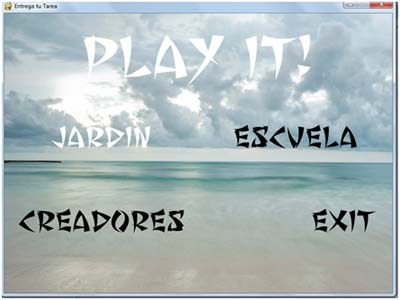
\includegraphics[width=0.7\textwidth]{principal.jpg}
		\end{center}
	\end{frame}
	\begin{frame}
		\begin{itemize}
			\item\textbf{NIVEL JARDIN}
			\pause
		\end{itemize}
		\begin{center} 
			 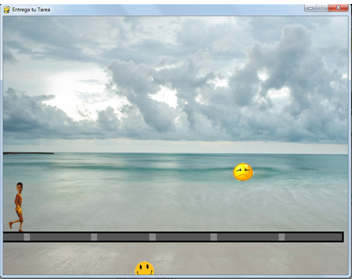
\includegraphics[width=0.7\textwidth]{nivel_jardin.png}
		\end{center}
	\end{frame}
	\begin{frame}
		\begin{itemize}
			\item\textbf{NIVEL ESCUELA}
			\pause
		\end{itemize}
		\begin{center} 
			 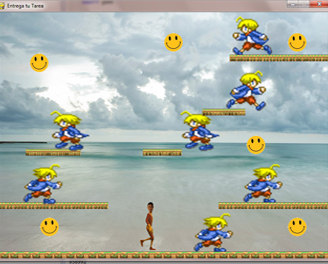
\includegraphics[width=0.7\textwidth]{nivel_escuela.png}
		\end{center}
	\end{frame}
	\begin{frame}
		\begin{center} 
			 
\includegraphics[width=0.9\textwidth]{gracias.jpg}
		\end{center}
	\end{frame}


\end{document}

